% Generated by scripts/rerun/make_figures.py - do not edit by hand.
\resizebox{\linewidth}{!}{%
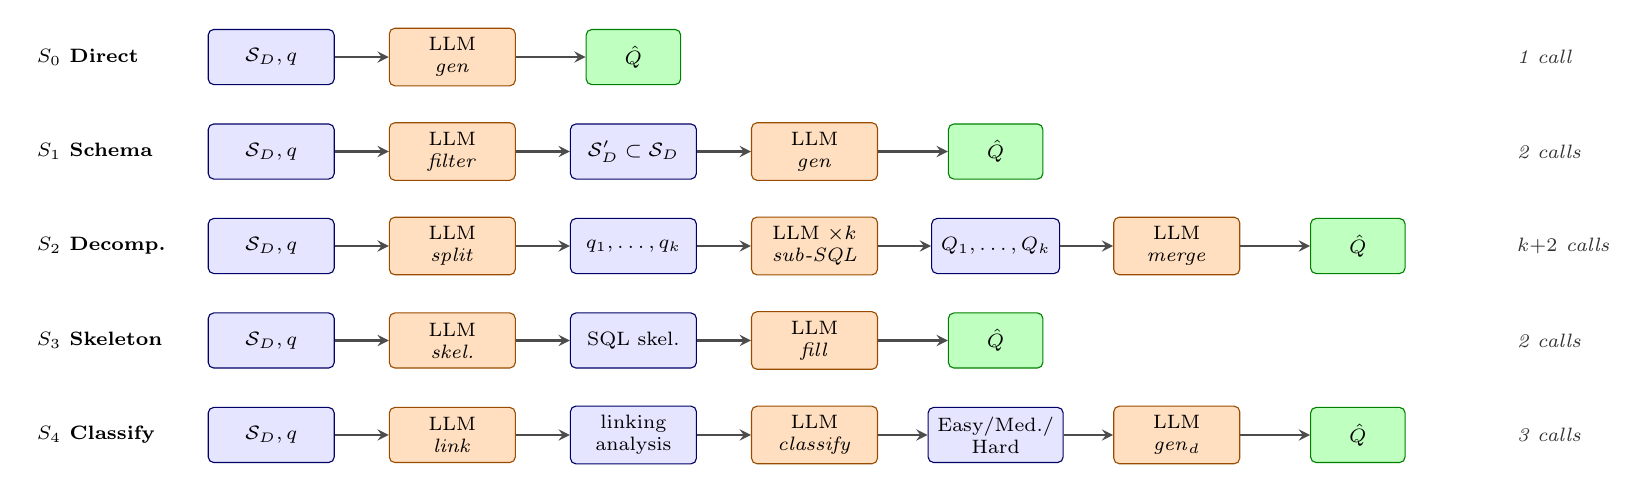
\begin{tikzpicture}[
    box/.style={draw=blue!40!black, rounded corners=2pt, minimum width=16mm, minimum height=7mm,
                align=center, font=\scriptsize, fill=blue!10},
    llm/.style={draw=orange!60!black, rounded corners=2pt, minimum width=16mm, minimum height=7mm,
                align=center, font=\scriptsize, fill=orange!25},
    outbox/.style={draw=green!50!black, rounded corners=2pt, minimum width=12mm, minimum height=7mm,
                align=center, font=\scriptsize, fill=green!25},
    lbl/.style={font=\scriptsize\bfseries, anchor=west},
    note/.style={font=\scriptsize\itshape, anchor=west, gray!40!black},
    arr/.style={->, >=stealth, thick, gray!60!black},
]
\def\cA{0}\def\cB{2.3}\def\cC{4.6}\def\cD{6.9}\def\cE{9.2}\def\cF{11.5}\def\cG{13.8}\def\cH{15.7}
\foreach \y/\name in {0/$S_0$ Direct, -1.2/$S_1$ Schema, -2.4/$S_2$ Decomp., -3.6/$S_3$ Skeleton, -4.8/$S_4$ Classify}{
  \node[lbl] at (-3.1,\y) {\name};
}
% S0
\node[box] (a0) at (\cA,0) {$\mathcal{S}_D, q$}; \node[llm] (b0) at (\cB,0) {LLM\\\textit{gen}}; \node[outbox] (c0) at (\cC,0) {$\hat{Q}$};
\draw[arr] (a0)--(b0); \draw[arr] (b0)--(c0); \node[note] at (\cH,0) {1 call};
% S1
\node[box] (a1) at (\cA,-1.2) {$\mathcal{S}_D, q$}; \node[llm] (b1) at (\cB,-1.2) {LLM\\\textit{filter}};
\node[box] (c1) at (\cC,-1.2) {$\mathcal{S}_D'\subset\mathcal{S}_D$}; \node[llm] (d1) at (\cD,-1.2) {LLM\\\textit{gen}}; \node[outbox] (e1) at (\cE,-1.2) {$\hat{Q}$};
\draw[arr] (a1)--(b1); \draw[arr] (b1)--(c1); \draw[arr] (c1)--(d1); \draw[arr] (d1)--(e1); \node[note] at (\cH,-1.2) {2 calls};
% S2
\node[box] (a2) at (\cA,-2.4) {$\mathcal{S}_D, q$}; \node[llm] (b2) at (\cB,-2.4) {LLM\\\textit{split}};
\node[box] (c2) at (\cC,-2.4) {$q_1,\ldots,q_k$}; \node[llm] (d2) at (\cD,-2.4) {LLM $\times k$\\\textit{sub-SQL}};
\node[box] (e2) at (\cE,-2.4) {$Q_1,\ldots,Q_k$}; \node[llm] (f2) at (\cF,-2.4) {LLM\\\textit{merge}}; \node[outbox] (g2) at (\cG,-2.4) {$\hat{Q}$};
\draw[arr] (a2)--(b2); \draw[arr] (b2)--(c2); \draw[arr] (c2)--(d2); \draw[arr] (d2)--(e2); \draw[arr] (e2)--(f2); \draw[arr] (f2)--(g2);
\node[note] at (\cH,-2.4) {$k{+}2$ calls};
% S3
\node[box] (a3) at (\cA,-3.6) {$\mathcal{S}_D, q$}; \node[llm] (b3) at (\cB,-3.6) {LLM\\\textit{skel.}};
\node[box] (c3) at (\cC,-3.6) {SQL skel.}; \node[llm] (d3) at (\cD,-3.6) {LLM\\\textit{fill}}; \node[outbox] (e3) at (\cE,-3.6) {$\hat{Q}$};
\draw[arr] (a3)--(b3); \draw[arr] (b3)--(c3); \draw[arr] (c3)--(d3); \draw[arr] (d3)--(e3); \node[note] at (\cH,-3.6) {2 calls};
% S4
\node[box] (a4) at (\cA,-4.8) {$\mathcal{S}_D, q$}; \node[llm] (b4) at (\cB,-4.8) {LLM\\\textit{link}};
\node[box] (c4) at (\cC,-4.8) {linking\\analysis}; \node[llm] (d4) at (\cD,-4.8) {LLM\\\textit{classify}};
\node[box] (e4) at (\cE,-4.8) {Easy/Med./\\Hard}; \node[llm] (f4) at (\cF,-4.8) {LLM\\\textit{gen}$_d$}; \node[outbox] (g4) at (\cG,-4.8) {$\hat{Q}$};
\draw[arr] (a4)--(b4); \draw[arr] (b4)--(c4); \draw[arr] (c4)--(d4); \draw[arr] (d4)--(e4); \draw[arr] (e4)--(f4); \draw[arr] (f4)--(g4);
\node[note] at (\cH,-4.8) {3 calls};
\end{tikzpicture}}
